%%%%%%%%%%%%%%%%%%%%%%%%%%%%%%%%%%%%%%%%%
% Short Sectioned Assignment
% LaTeX Template
% Version 1.0 (5/5/12)
%
% This template has been downloaded from:
% http://www.LaTeXTemplates.com
%
% Original author:
% Frits Wenneker (http://www.howtotex.com)
%
% License:
% CC BY-NC-SA 3.0 (http://creativecommons.org/licenses/by-nc-sa/3.0/)
%
%%%%%%%%%%%%%%%%%%%%%%%%%%%%%%%%%%%%%%%%%

%----------------------------------------------------------------------------------------
%	PACKAGES AND OTHER DOCUMENT CONFIGURATIONS
%----------------------------------------------------------------------------------------

\documentclass[paper=a4, fontsize=11pt]{scrartcl} % A4 paper and 11pt font size

\usepackage{comment}
\usepackage[T1]{fontenc} % Use 8-bit encoding that has 256 glyphs
\usepackage{fourier} % Use the Adobe Utopia font for the document - comment this line to return to the LaTeX default
\usepackage[english]{babel} % English language/hyphenation
\usepackage{amsmath,amsfonts,amsthm} % Math packages

\usepackage{lipsum} % Used for inserting dummy 'Lorem ipsum' text into the template
\usepackage{graphicx}

\usepackage{sectsty} % Allows customizing section commands
\allsectionsfont{\centering \normalfont\scshape} % Make all sections centered, the default font and small caps

\usepackage{fancyhdr} % Custom headers and footers
\pagestyle{fancyplain} % Makes all pages in the document conform to the custom headers and footers
\fancyhead{} % No page header - if you want one, create it in the same way as the footers below
\fancyfoot[L]{} % Empty left footer
\fancyfoot[C]{} % Empty center footer
\fancyfoot[R]{\thepage} % Page numbering for right footer
\renewcommand{\headrulewidth}{0pt} % Remove header underlines
\renewcommand{\footrulewidth}{0pt} % Remove footer underlines
\setlength{\headheight}{13.6pt} % Customize the height of the header

\numberwithin{equation}{section} % Number equations within sections (i.e. 1.1, 1.2, 2.1, 2.2 instead of 1, 2, 3, 4)
\numberwithin{figure}{section} % Number figures within sections (i.e. 1.1, 1.2, 2.1, 2.2 instead of 1, 2, 3, 4)
\numberwithin{table}{section} % Number tables within sections (i.e. 1.1, 1.2, 2.1, 2.2 instead of 1, 2, 3, 4)

\setlength\parindent{0pt} % Removes all indentation from paragraphs - comment this line for an assignment with lots of text

%----------------------------------------------------------------------------------------
%	TITLE SECTION
%----------------------------------------------------------------------------------------

\newcommand{\horrule}[1]{\rule{\linewidth}{#1}} % Create horizontal rule command with 1 argument of height

\title{	
\normalfont \normalsize 
\textsc{La Sapienza University of Rome. Department of Computer, Control, and Management Engineering} \\ [25pt] % Your university, school and/or department name(s)
\horrule{0.5pt} \\[0.4cm] % Thin top horizontal rule
\huge Interactive Graphics Final Project \\ % The assignment title
\horrule{2pt} \\[0.5cm] % Thick bottom horizontal rule
}

\author{Jean Pierre Richa, Simone Faricelli} % Your name

\date{\normalsize\today} % Today's date or a custom date

\begin{document}
\maketitle % Print the title
%----------------------------------------------------------------------------------------
%	PROBLEM 1
%----------------------------------------------------------------------------------------

\section{Introduction}

The project is about creating a game we named FishIt see figure \ref{world}, which is an interactive game made as close to reality as possible, it simulates a fisherman driving a boat inside a world consisting of everything that we can find in a real world fishing environment, such as the sky, sun, light-house, boat, rod, water, and fishes. The aim from the game is trying to catch as much fishes as possible. Each fish catches increases the total score by 1. \par We used rigid 3D objects, which we later animated using javascript such as the boat, and the rod, which can both be controlled by the user using the keyboard and the fishes, which move randomly in the water. Furthermore, we included a hierarchical structure, which we are going to see in details when we discuss the implementation. The hierarchical structure was applied on several objects such as the boat and the rod. The fishes move randomly and when the rod is thrown in the water, we wait for the bait to collide with a fish and give the user a counter specifying the time within which he should pull the rod to gain points, otherwise the fish will escape and he will not gain a new point.

\begin{figure}
\centering
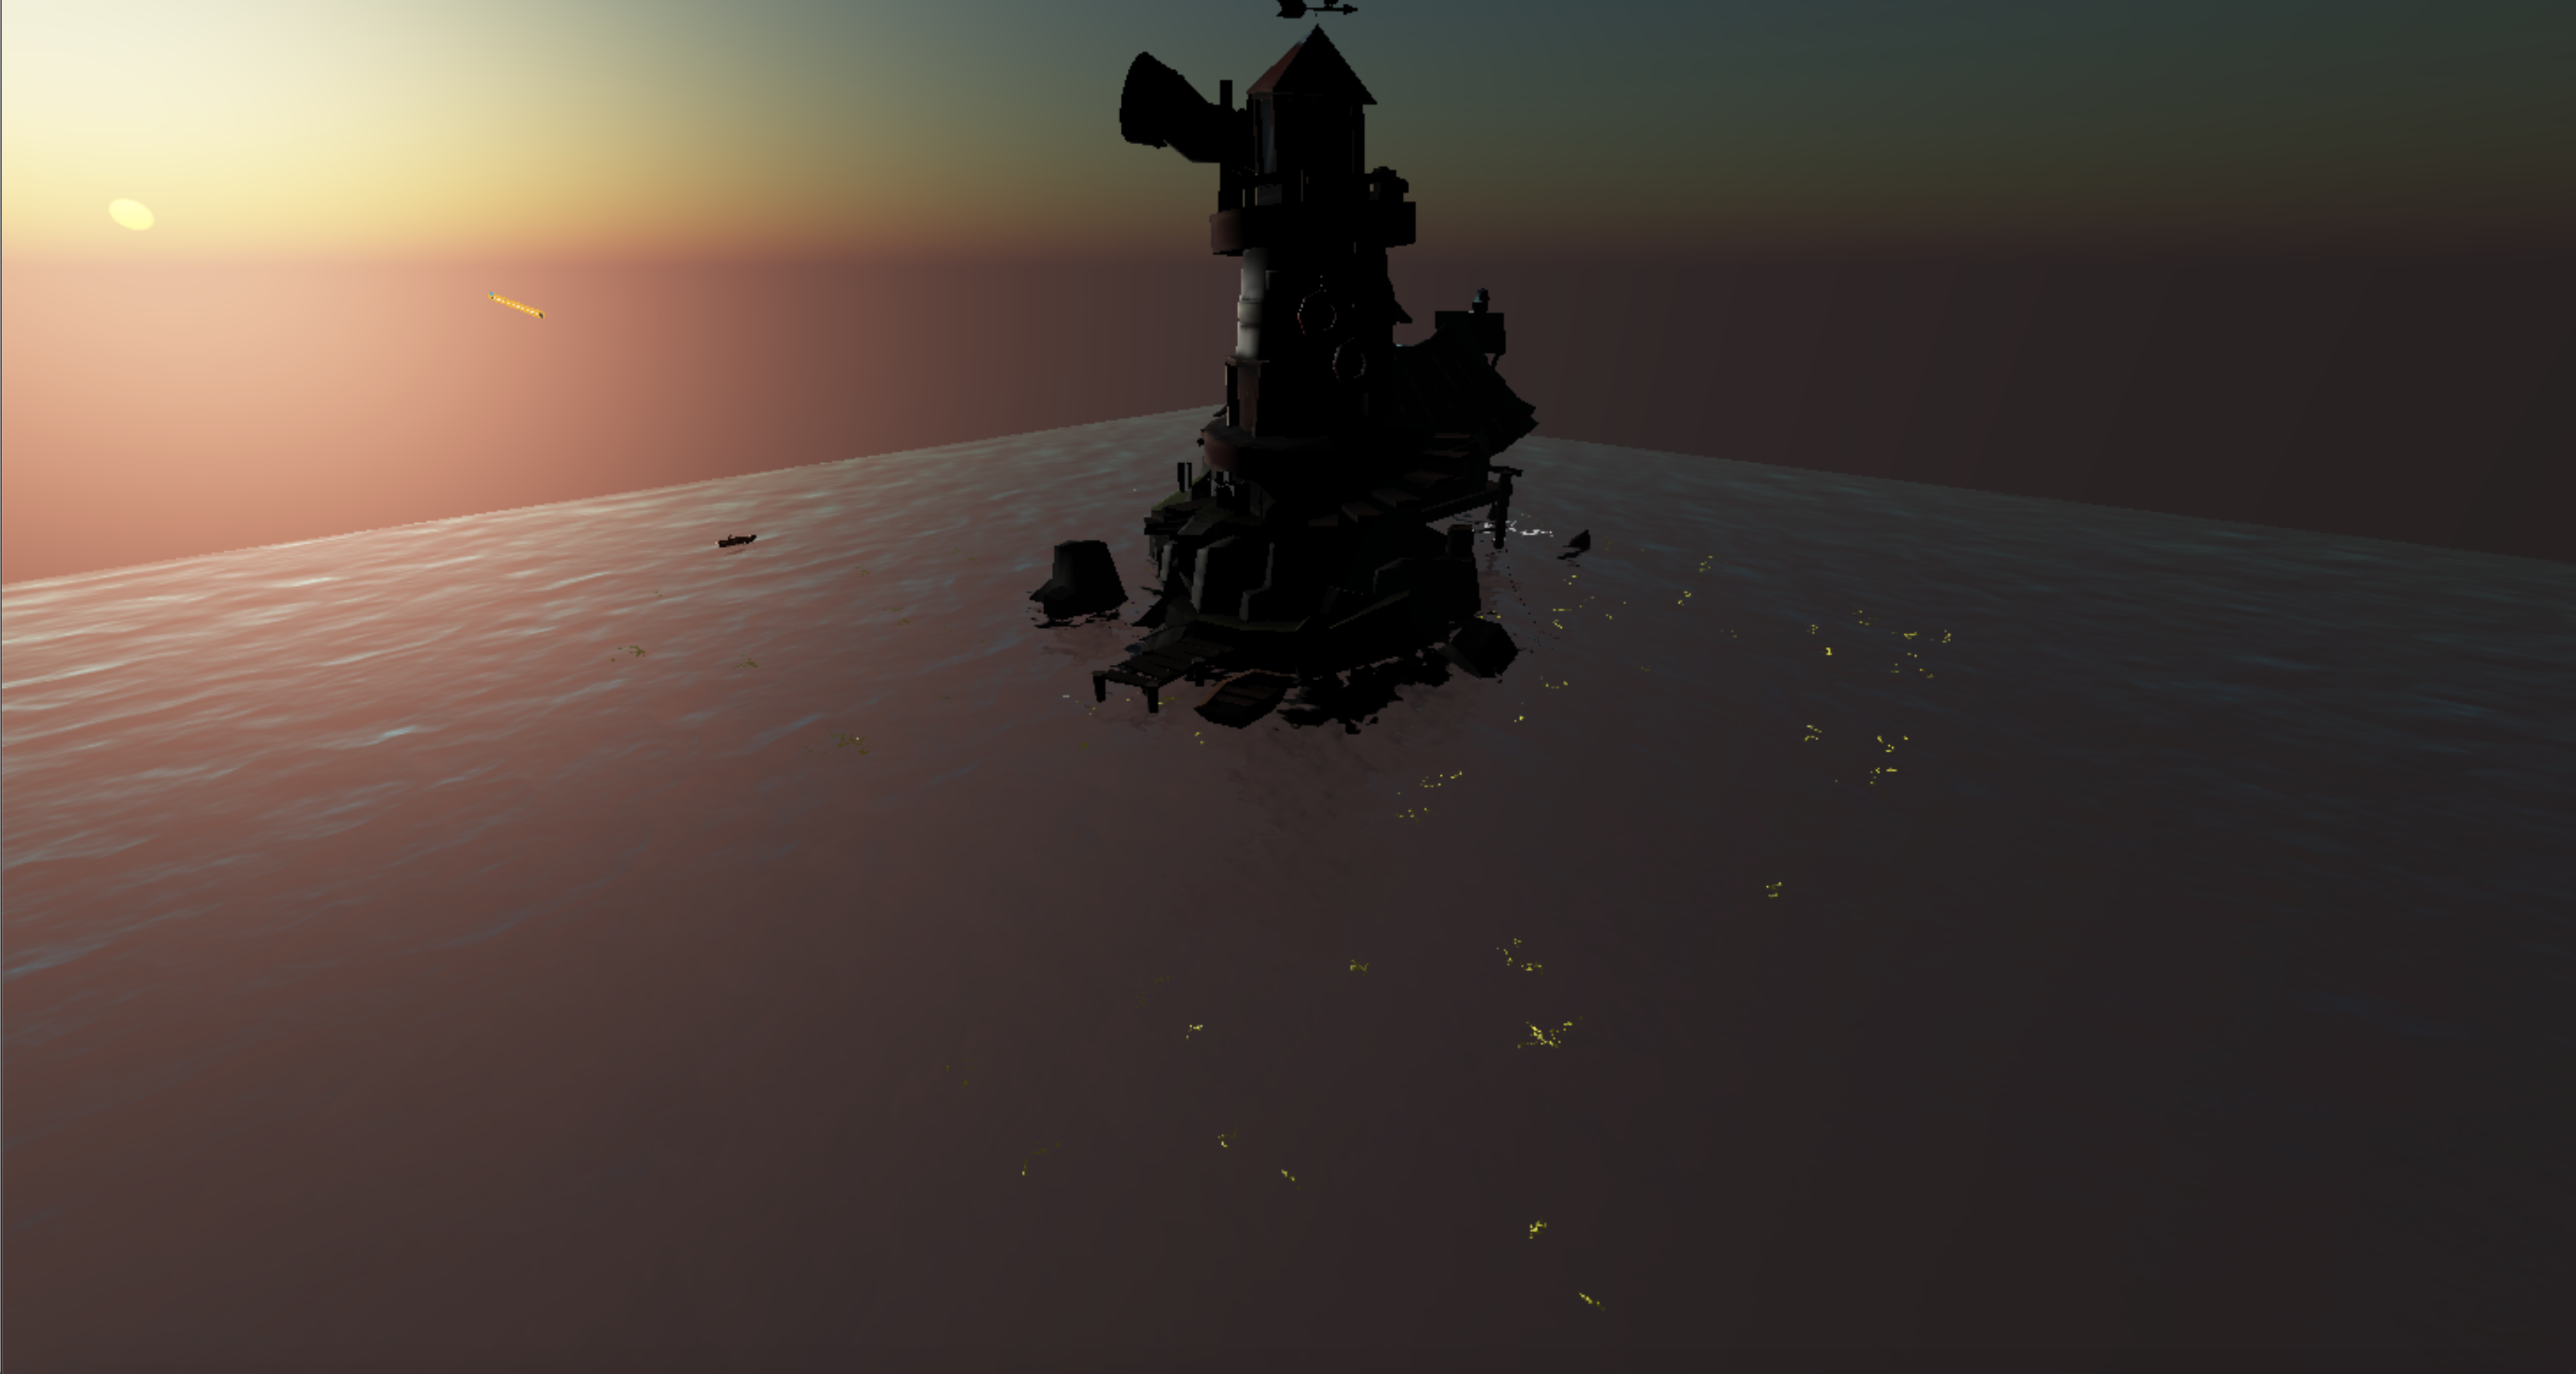
\includegraphics[width=15cm, height=7cm]{images/world.png}
\caption{Top view for the whole environment.}
\label{world}
\end{figure}

\newpage

%------------------------------------------------

%\subsection{Heading on level 2 (subsection)}
\section{Implementation}

In order to have a clear view about the implementation, this section will be split into several part, where each part will hold details about the implementation of each object. The areas that will be discussed in the following subsections are: the creation of each object, the placement in the environment, whether the object is controllable and how it is controllable, and other details specific to each object.

\subsection{Sky}

The first object to consider in this project is the sky, because we need the environment to look as real as possible. The sky meshes which hold the geometry of the object that consist of the vertices attributes were imported from three.js. After that, the turbidity, luminance, and other characteristics were specified for the sky to fit this specific environment. The sky is clear and fixed, and cannot be controlled. The turbidity and the other characteristics were chosen to make the daytime look like if it's near the sunset.

\subsection{Sun}

An important part of this project is the sun, because we need a light source. In order to have it, as in importing the sky, the sun meshes hold the geometry of the object , which were also imported from three.js, and then the object was added to the scene. After that, the position and visibility were specified for the sun. For better visualization check figure \ref{sun}.

\begin{figure}[!ht]
\centering
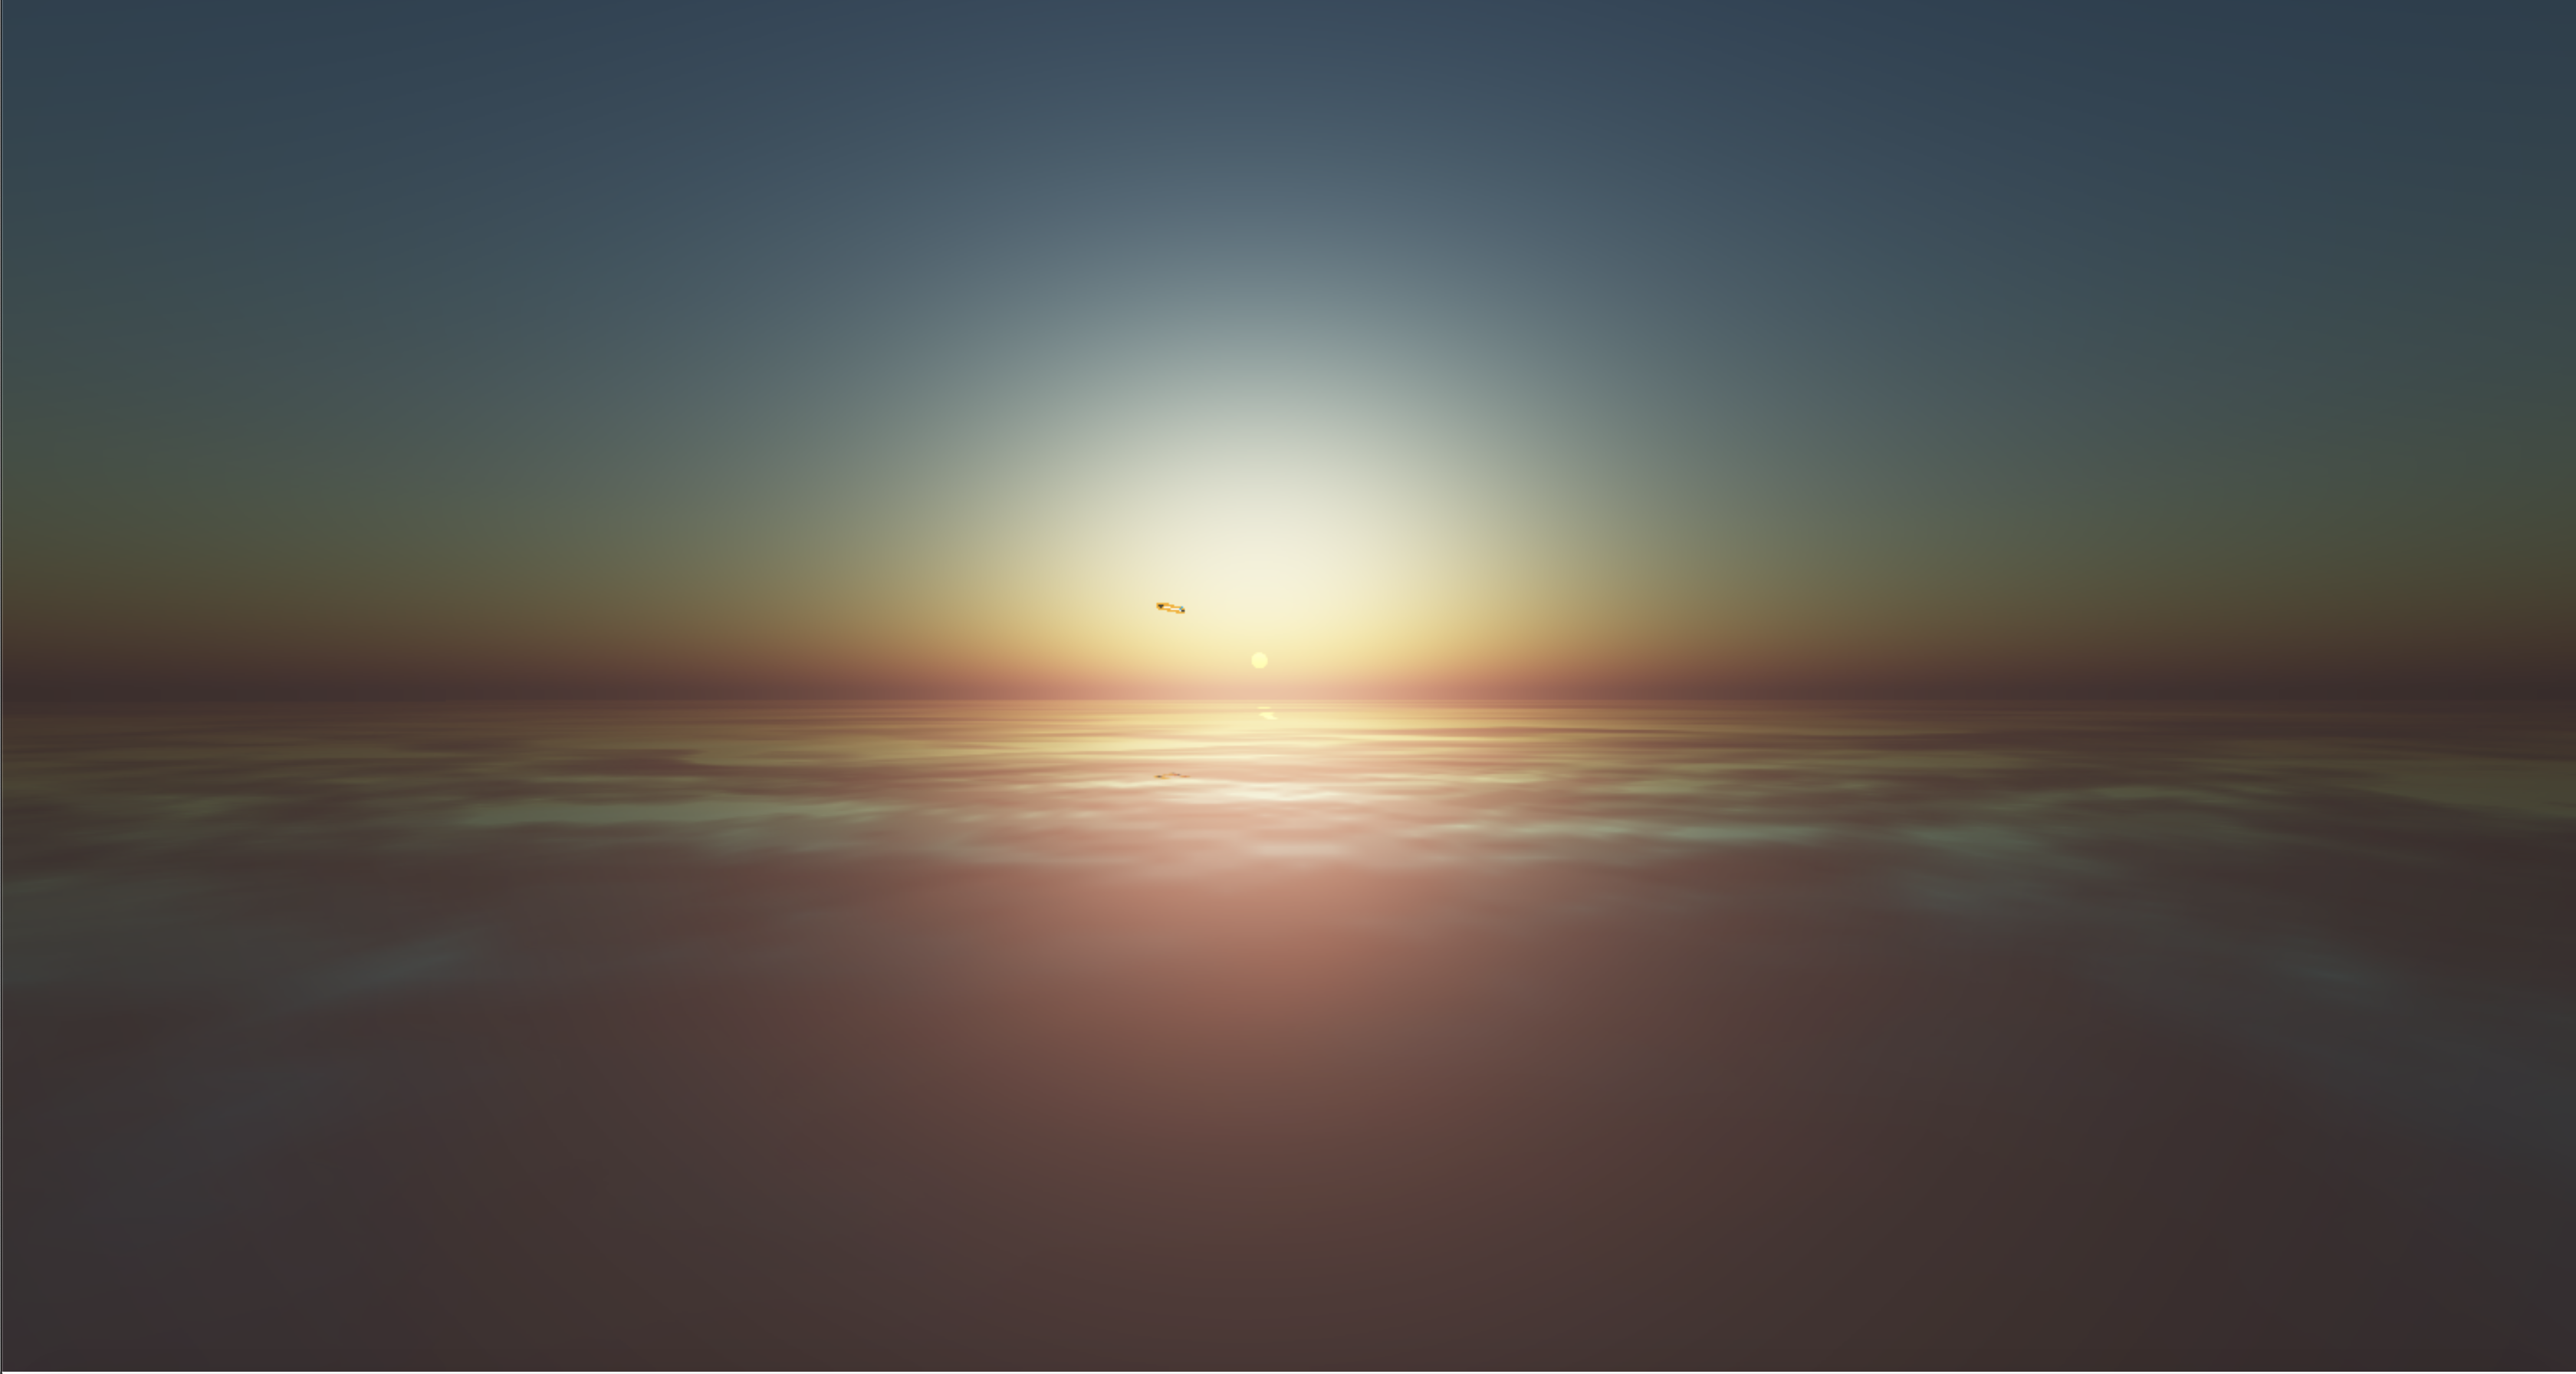
\includegraphics[width=15cm, height=7cm]{images/sun.png}
\caption{The sun viewed from the lake.}
\label{sun}
\end{figure}
\newpage

\subsection{Light}

Light is the main external element one have to deal with; For that, it was imported from three.js and its position was chosen according to the sun position, and orientation. An important issue to deal with when it comes to using lights in a scene is shadowing, so castShadow function for the light was set to true in order to get the objects in the environment rendered into the shadow map. The light ambiance was chosen to fit the time of the day, which is the sunset.

\subsection{Hierarchy}

A necessary feature is building a hierarchical structure. The structure is obtained through creating nodes in a hierarchical way where each node has a sibling and/or a child. The child is usually the node following the current one, and the sibling is the node parallel or next to the current one. The whole structure have to be aligned along a specific axis based on its desired position, because as we will see, sometimes an object should be below, next, or above the other one. First of all, and in order to have a clean implementation, we need to start by the central object, which is the lighthouse since the other moving objects will be turning around it. After creating all the nodes specifying whether it's a sibling or a child of another node, and specifying the location of the node using the parent's location, we will obtain all the parts connected to each other.

\subsection{3D Objects}

The approach for adding the different materials used in this project, is importing non-animated 3D objects such as the rod, boat, lighthouse, and fishes. See \ref{house} 
Using the hierarchical structure we can put different parts together, which in this case are the previously listed objects added to the environment scene. The main idea of using the hierarchy is to simplify the relation between the boat and the different parts of the rod (handle, rope, and bait), which were split to make it easier for the collision checking with the fishes. The boat was imported and then coded from scratch to be moved in the environment by the user. The rod can be thrown and pulled by the user also, but the trick here is to tell the user within which time frame the rod should be pulled after colliding with the fish and this was done using a counter that shows on the screen the slot within which the fish is still in collision with the bait. If the rod was pulled in this time frame, a point will be added to the final score. Otherwise, no points will be gained.\par
The boat can be driven using the keyboard keys:
\begin{itemize}
\item W for moving forward,
\item S for moving backward,
\item W + A for moving left forward,
\item W + D for moving right forward,
\item S + A for moving left backward,
\item S + D for moving right backward.
\item The rod can be thrown using "G" and pulled using "F" 
\end{itemize}


\begin{figure}[!ht]
\centering
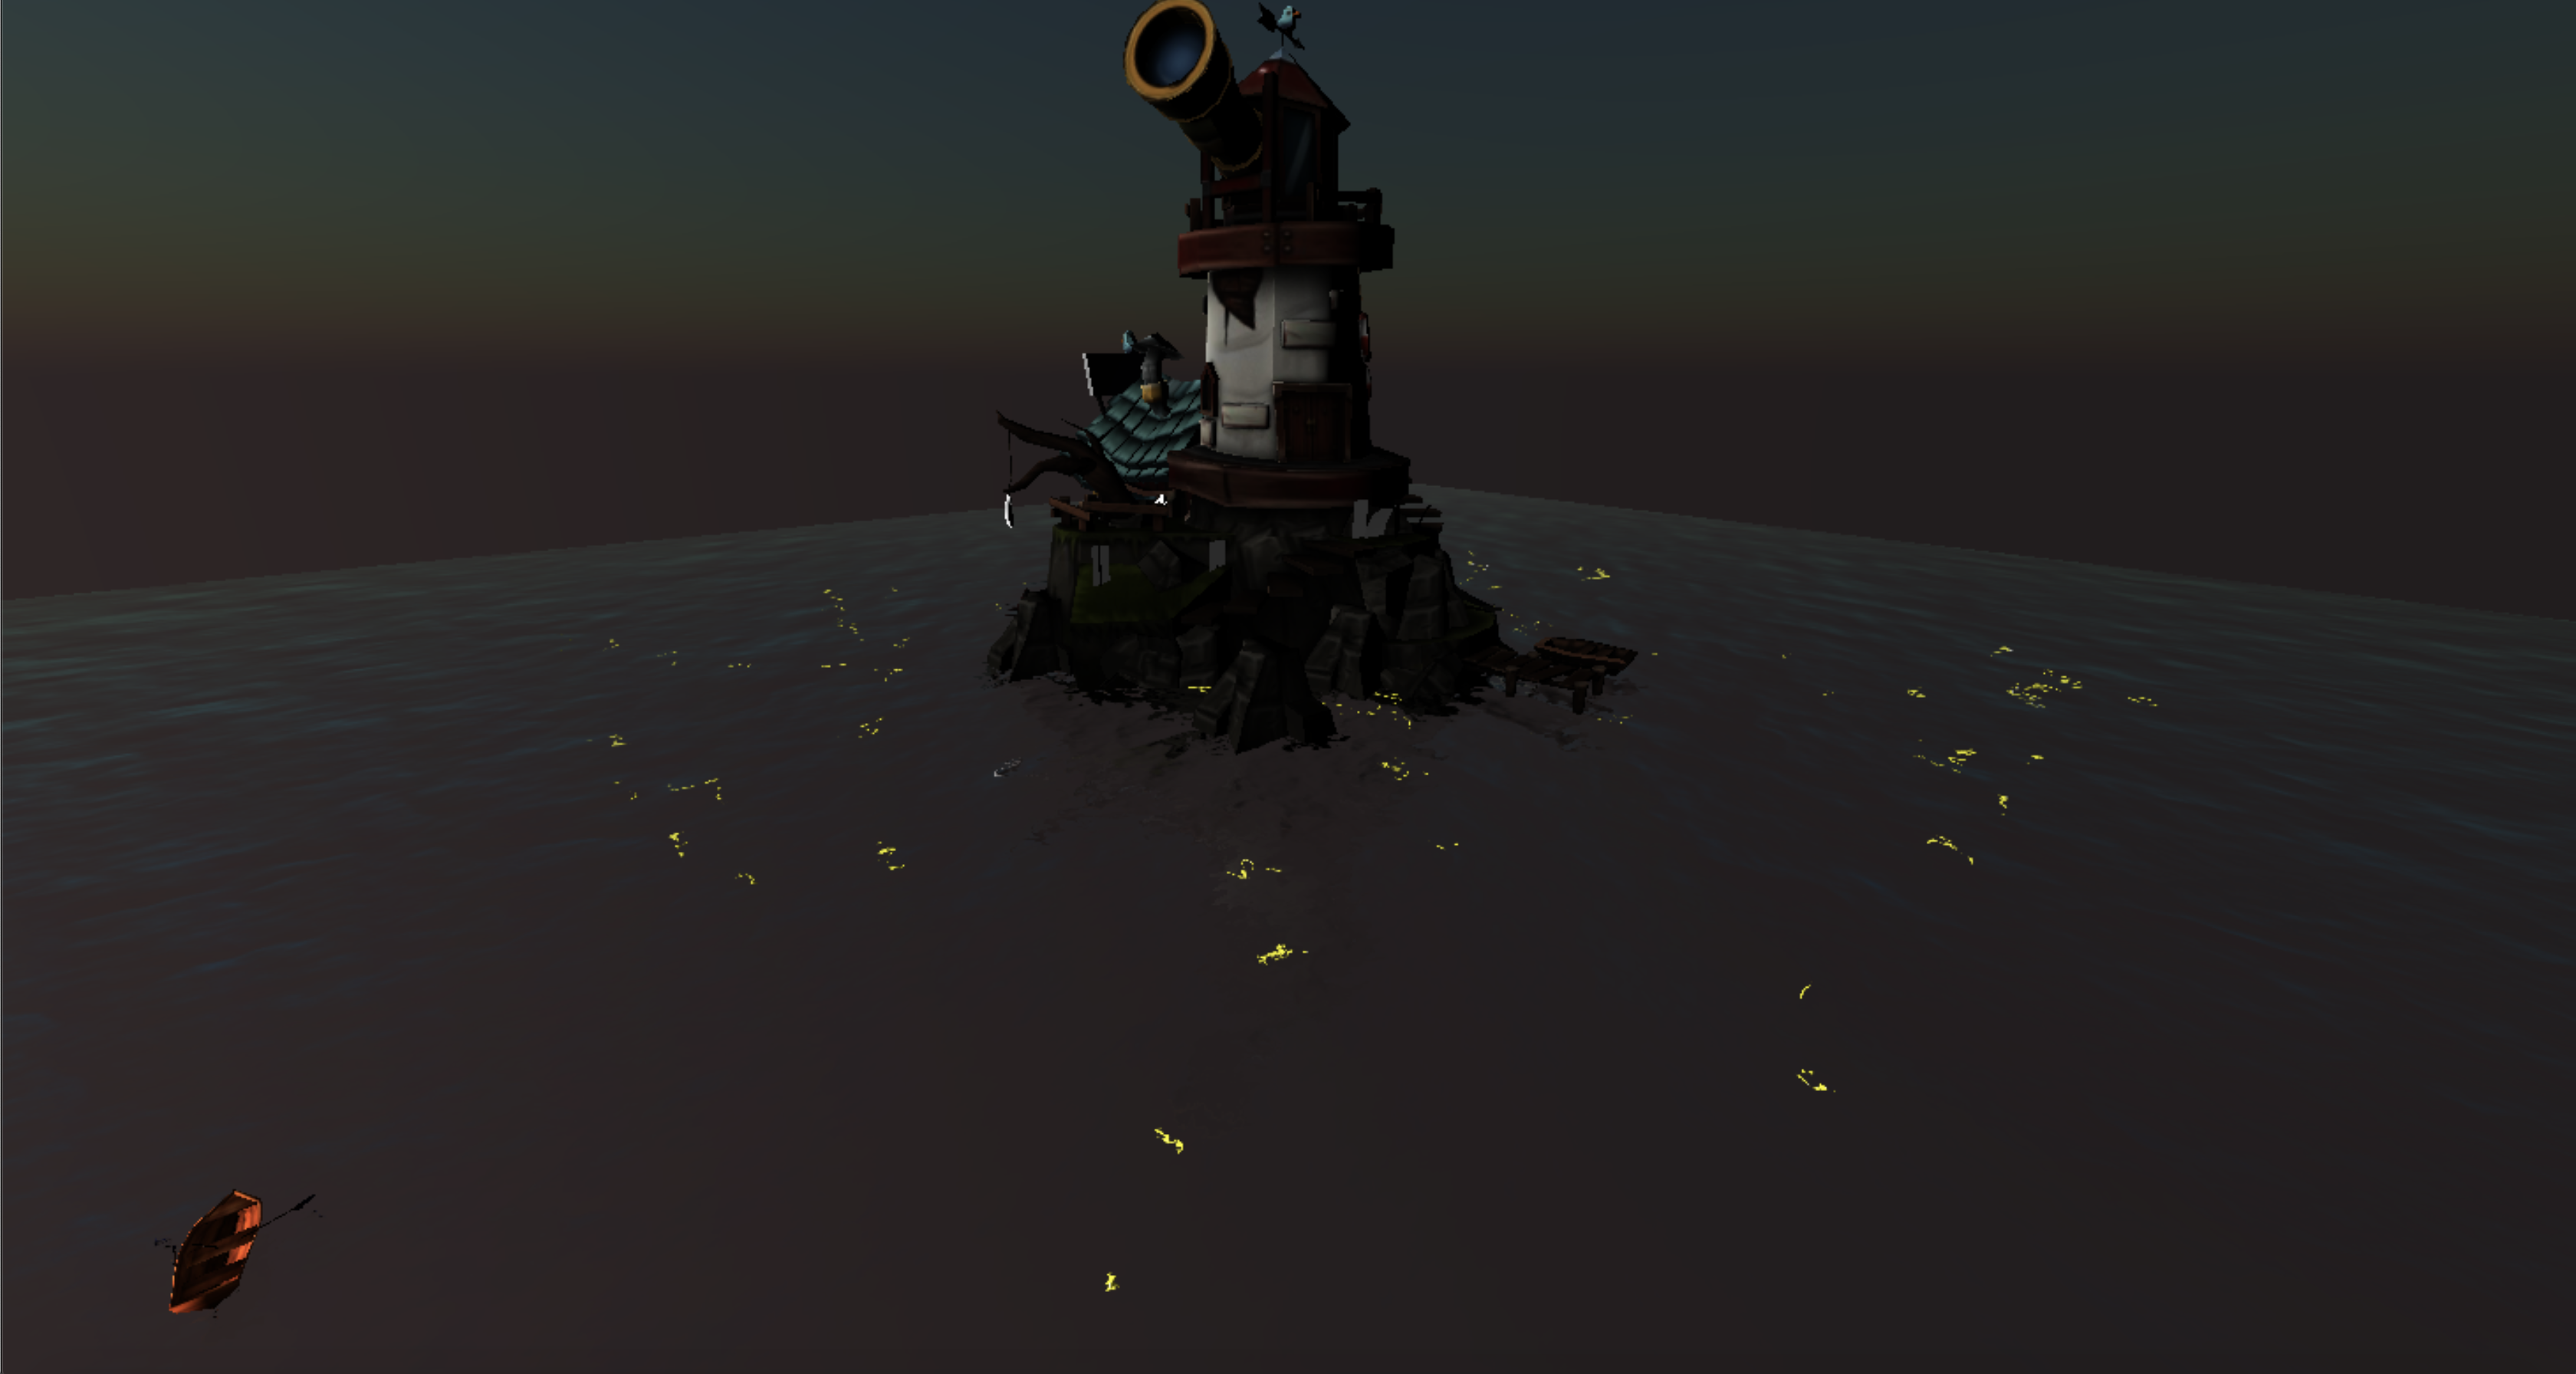
\includegraphics[width=15cm, height=7cm]{images/lighthouse.png}
\caption{View for all the objects.}
\label{house}
\end{figure}
\newpage

\subsection{Camera}

It is important for the user to see what is going on during the time he is playing, more specifically it is crucial to see everything relevant to getting a higher score, and knowing his/her position in the environment. In order to provide this feature, the camera was placed on the boat, where the view changes based on what the user is doing. For example if the user is driving the boat, the camera will show what's in front of it see \ref{boat view}, but when the driving stops, the camera will show the rod, so the user knows whether it is in the water or not see \ref{Drod} and \ref{Urod}.

\begin{figure}[!ht]
\centering
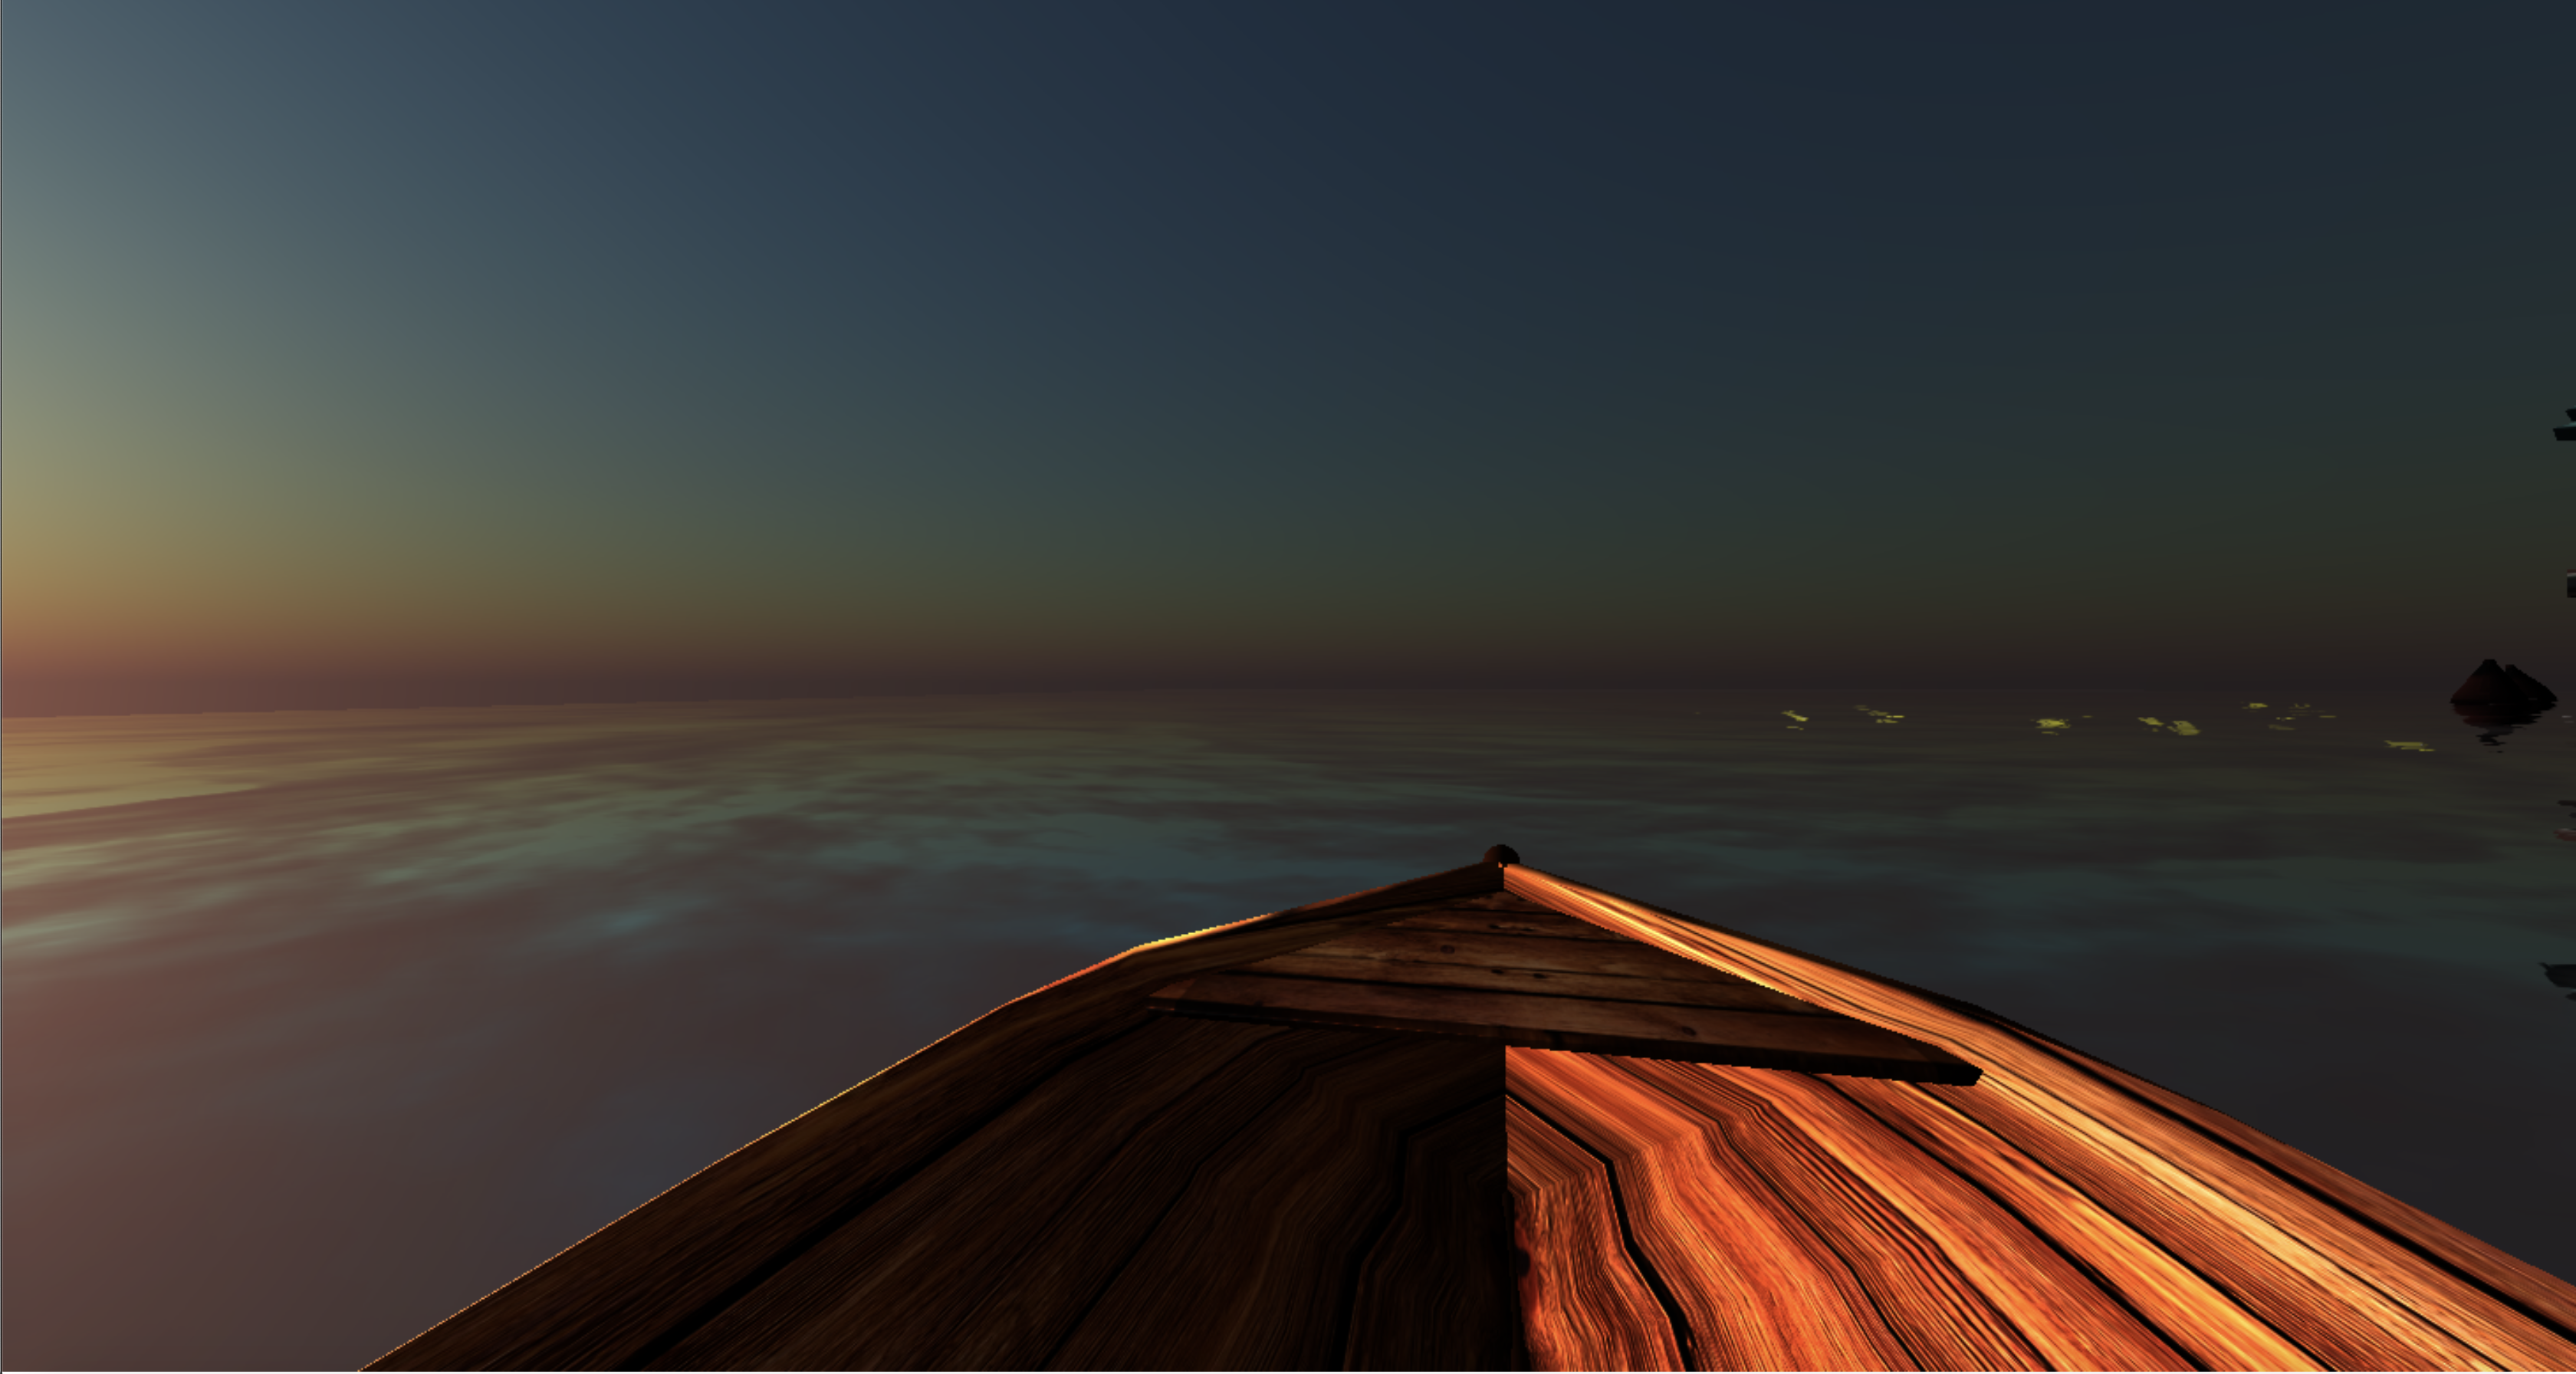
\includegraphics[width=15cm, height=7cm]{images/boatview.png}
\caption{Camera view while driving the boat}
\label{boat view}
\end{figure}

\begin{figure}[!ht]
\centering
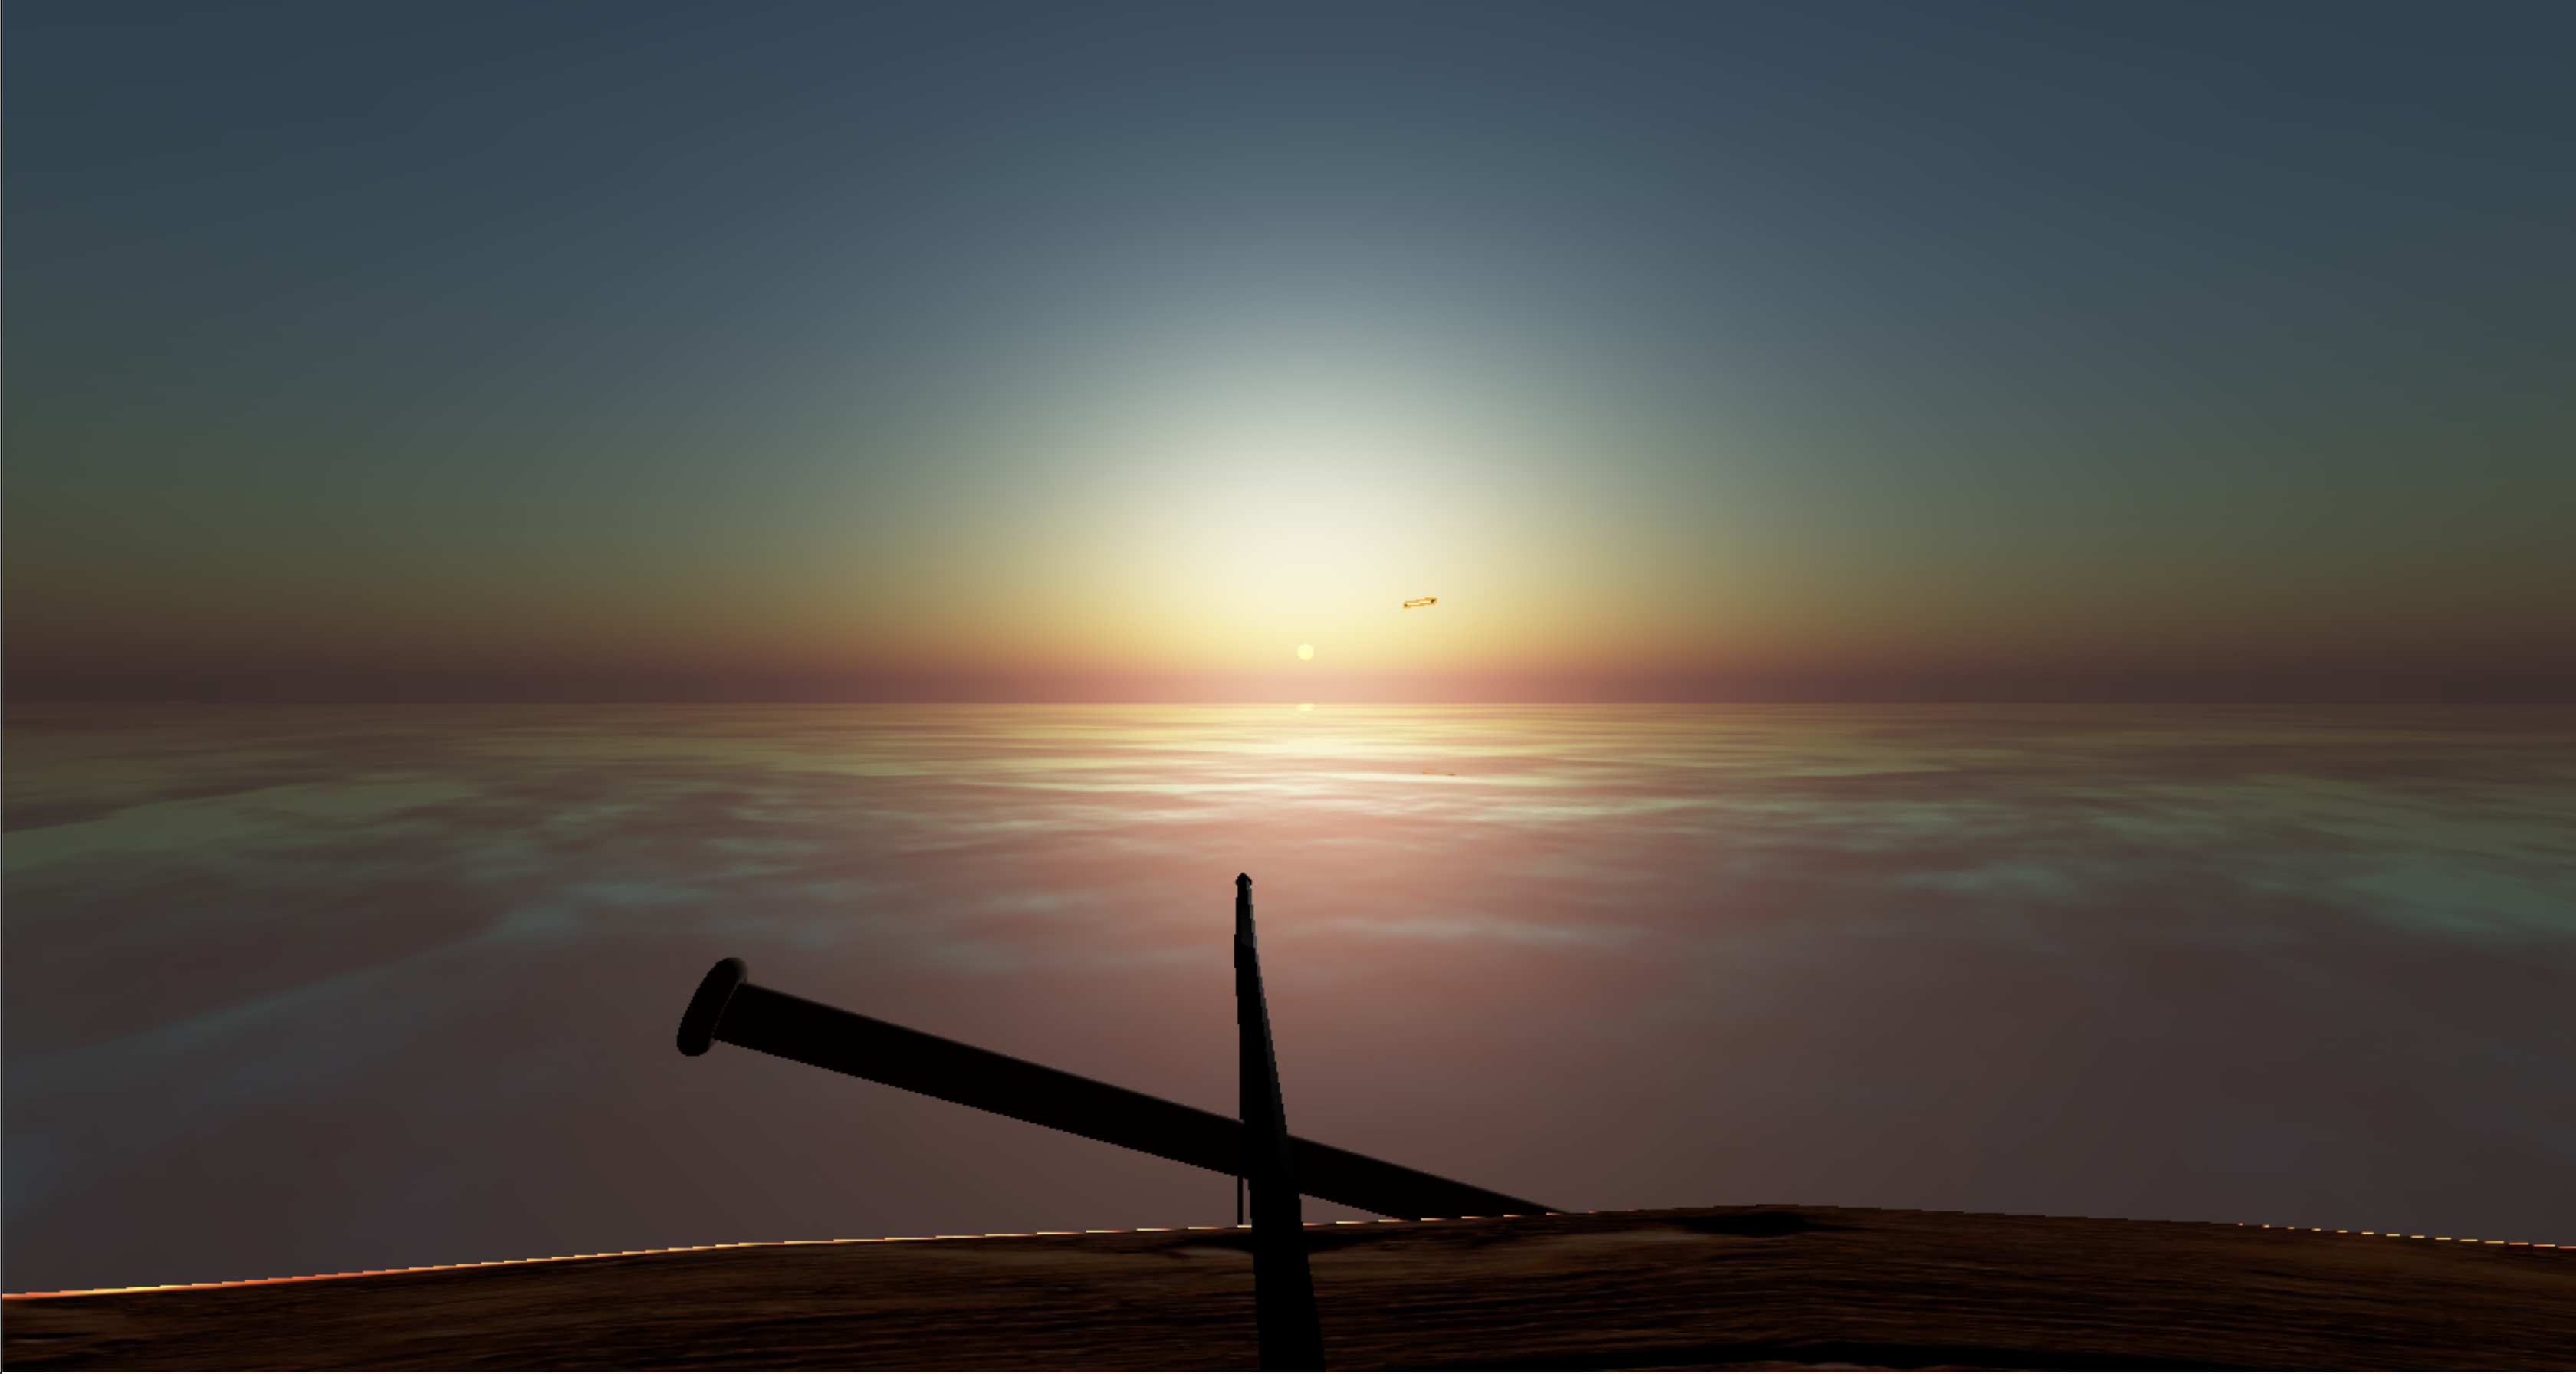
\includegraphics[width=15cm, height=7cm]{images/thrownrod.png}
\caption{Camera view when the rod is thrown and the user is not driving the boat.}
\label{Drod}
\end{figure}

\begin{figure}[!ht]
\centering
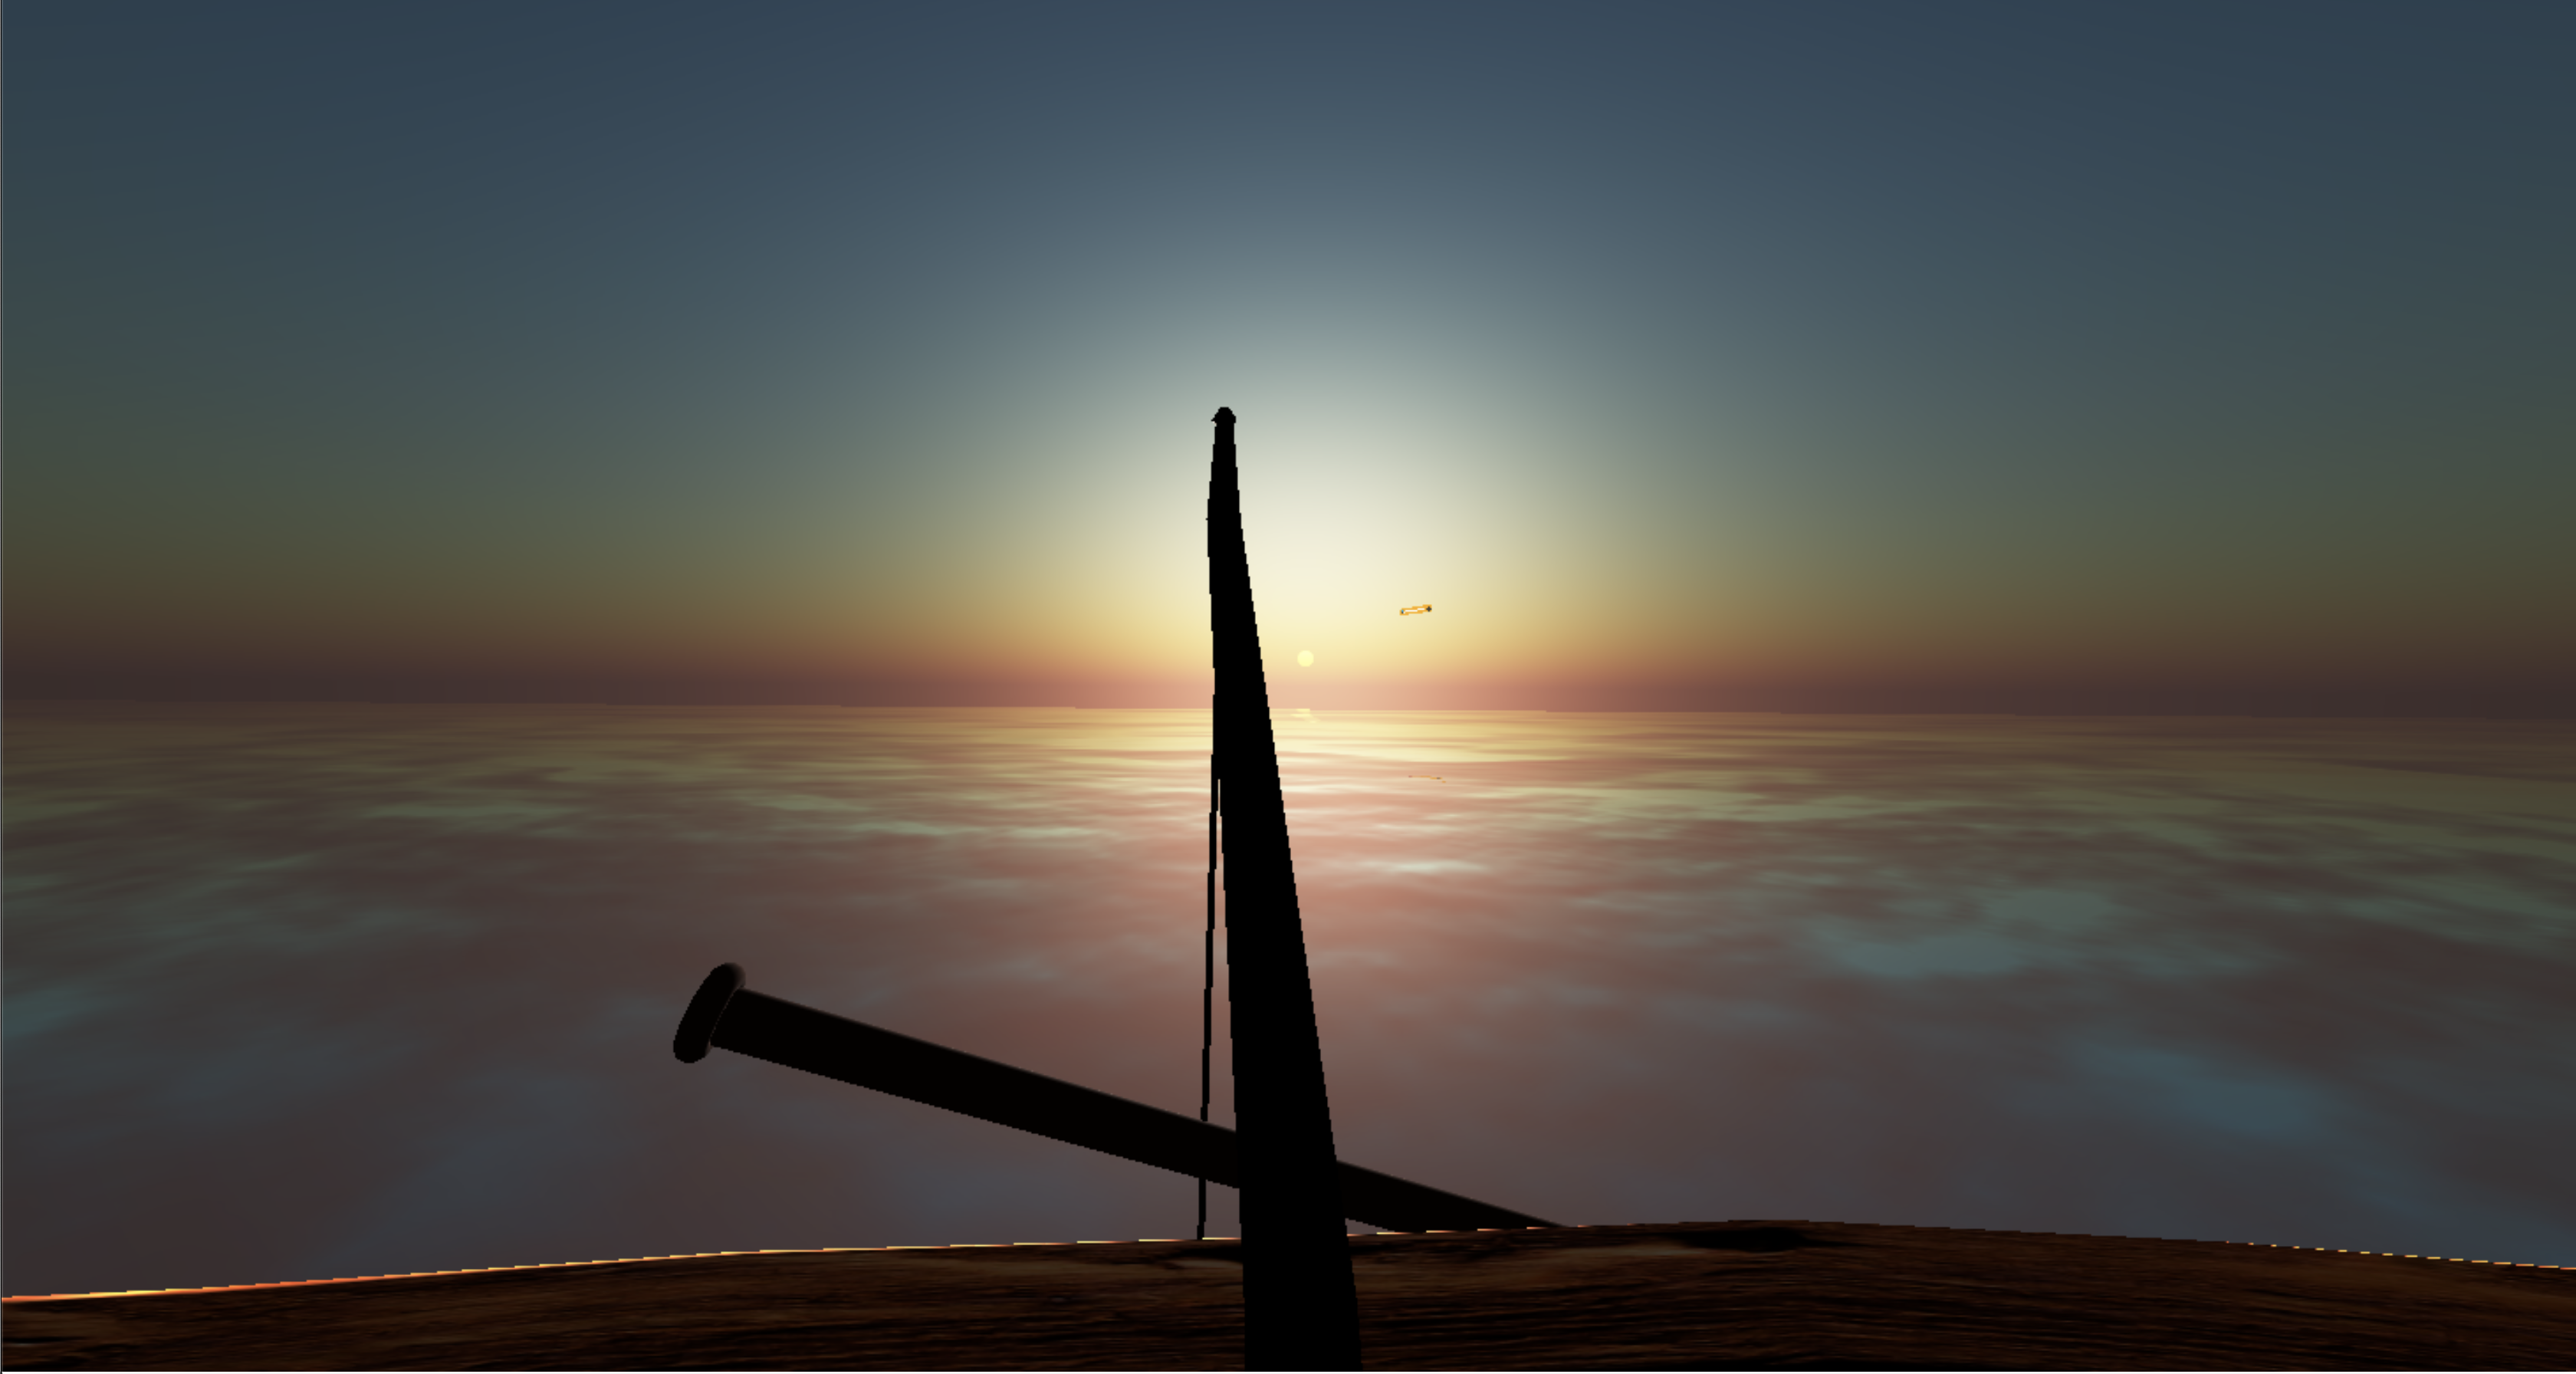
\includegraphics[width=15cm, height=7cm]{images/pulledrod.png}
\caption{Camera view when the rod is pulled and the user is not driving the boat.}
\label{Urod}
\end{figure}

\newpage
\subsection{Fishes}

A 3D model of a goldfish was imported and used, it was added to the scene a Hundred times, each with a different name. The fishes move randomly in the environment at a constant speed. They move randomly, in order to make it more difficult for the user to predict the next direction of the fish, which makes the game harder and the collision more difficult to happen. The fishes were put at a depth of 20 pixels below the water surface see \ref{fishes}, which is their fixed depth. 

\begin{figure}[!ht]
\centering
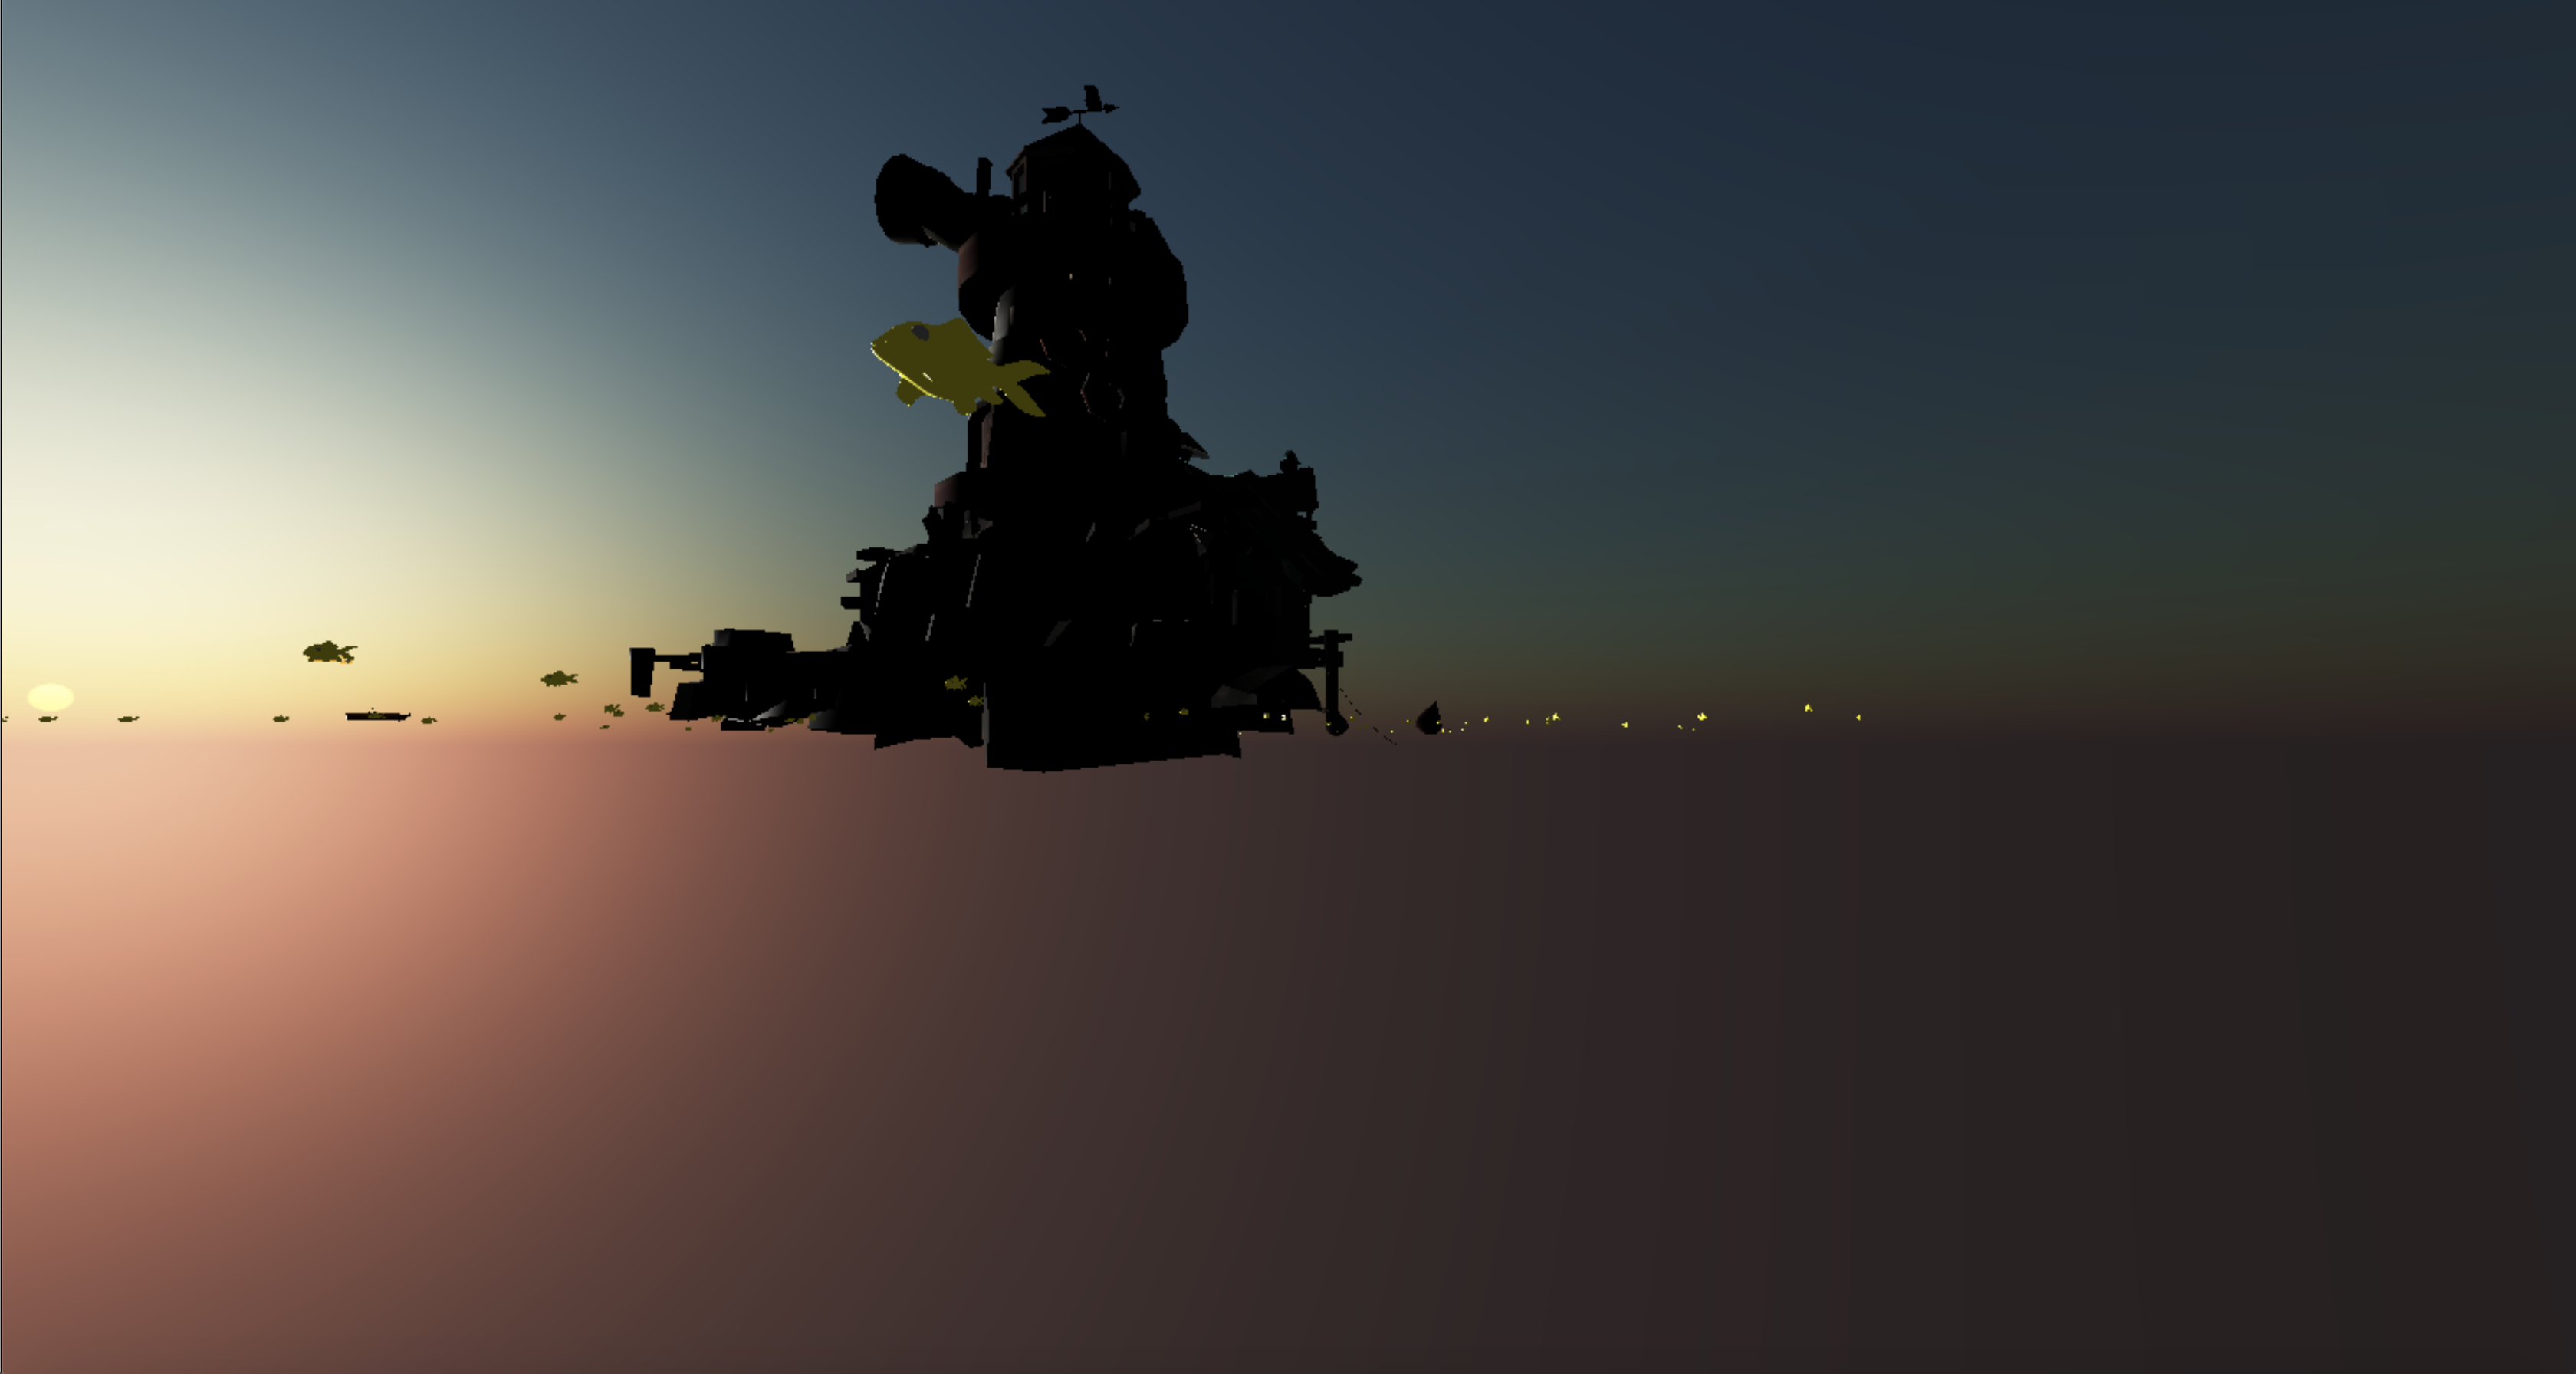
\includegraphics[width=15cm, height=7cm]{images/fishes.png}
\caption{Fishes view from underneath the water.}
\label{fishes}
\end{figure}

\subsection{Collison}

In order for a collision between the bait and a fish to happen, then the bait and the fish should be at the same height on the Y axis, which is 20 pixels below the water surface as previously stated. Because the vertical axis here is Y, since we are using three.js and this is the reference frame orientation in this library. they also should be on the same X, and Z axes points.

\section{Launching the game}

For the application to run, we need first to establish a local server, which can be done using python through navigating to the game's directory using the command prompt (terminal shell) and writing: "python -m http.server". After the connection is established, one can open a browser and type "localhost:8000", this will allow the game to load in the browser page.

\section{Third Party}

THREE.js: all the object were imported using THREE.js. Sun, sky and water were imported from THREE.js
\\~\\
Sketchfab: it was used to download the 3D objects, such as the boat, rod, fishes, and lighthouse.
\\~\\
Blender: was used to correct the the reference frames of the objects and the orientation and then exported to be imported inside the game using THREE.js
\end{document}